\section{Design}
Design dell'architettura del sistema e delle interfacce Utente

\subsection{Metodologie di sviluppo}
La prima fase di design si è concentrata nella definizione delle metodologie di sviluppo in team, in questo caso composto da 3 persone.

L'obiettivo è stato quello di lavorare in modalità \textbf{Agile}, scomponendo tutto il progetto in piccoli task, 
ognuno dei quali era scelto e preso in carico da un membro in accordo con gli altri a seconda delle priorità.

Settimanalmente è stato fatto il punto della situazione attraverso video conferenze su Google Meet, 
ogni membro del team era aggiornato sullo stato dei task, le difficoltà risontrate, i problemi risolti e le decisioni prese.
In questa fase veniva aggiornato lo stato dei task (\textbf{To Do}, \textbf{Doing}, \textbf{Done}), 
eventualmente aggiunti o modificati in base alle esigenze emerse
e si proseguiva scegliendo nuovamente i prossimi step da realizzare per avanzare.

\begin{figure}[H]
	\centering
	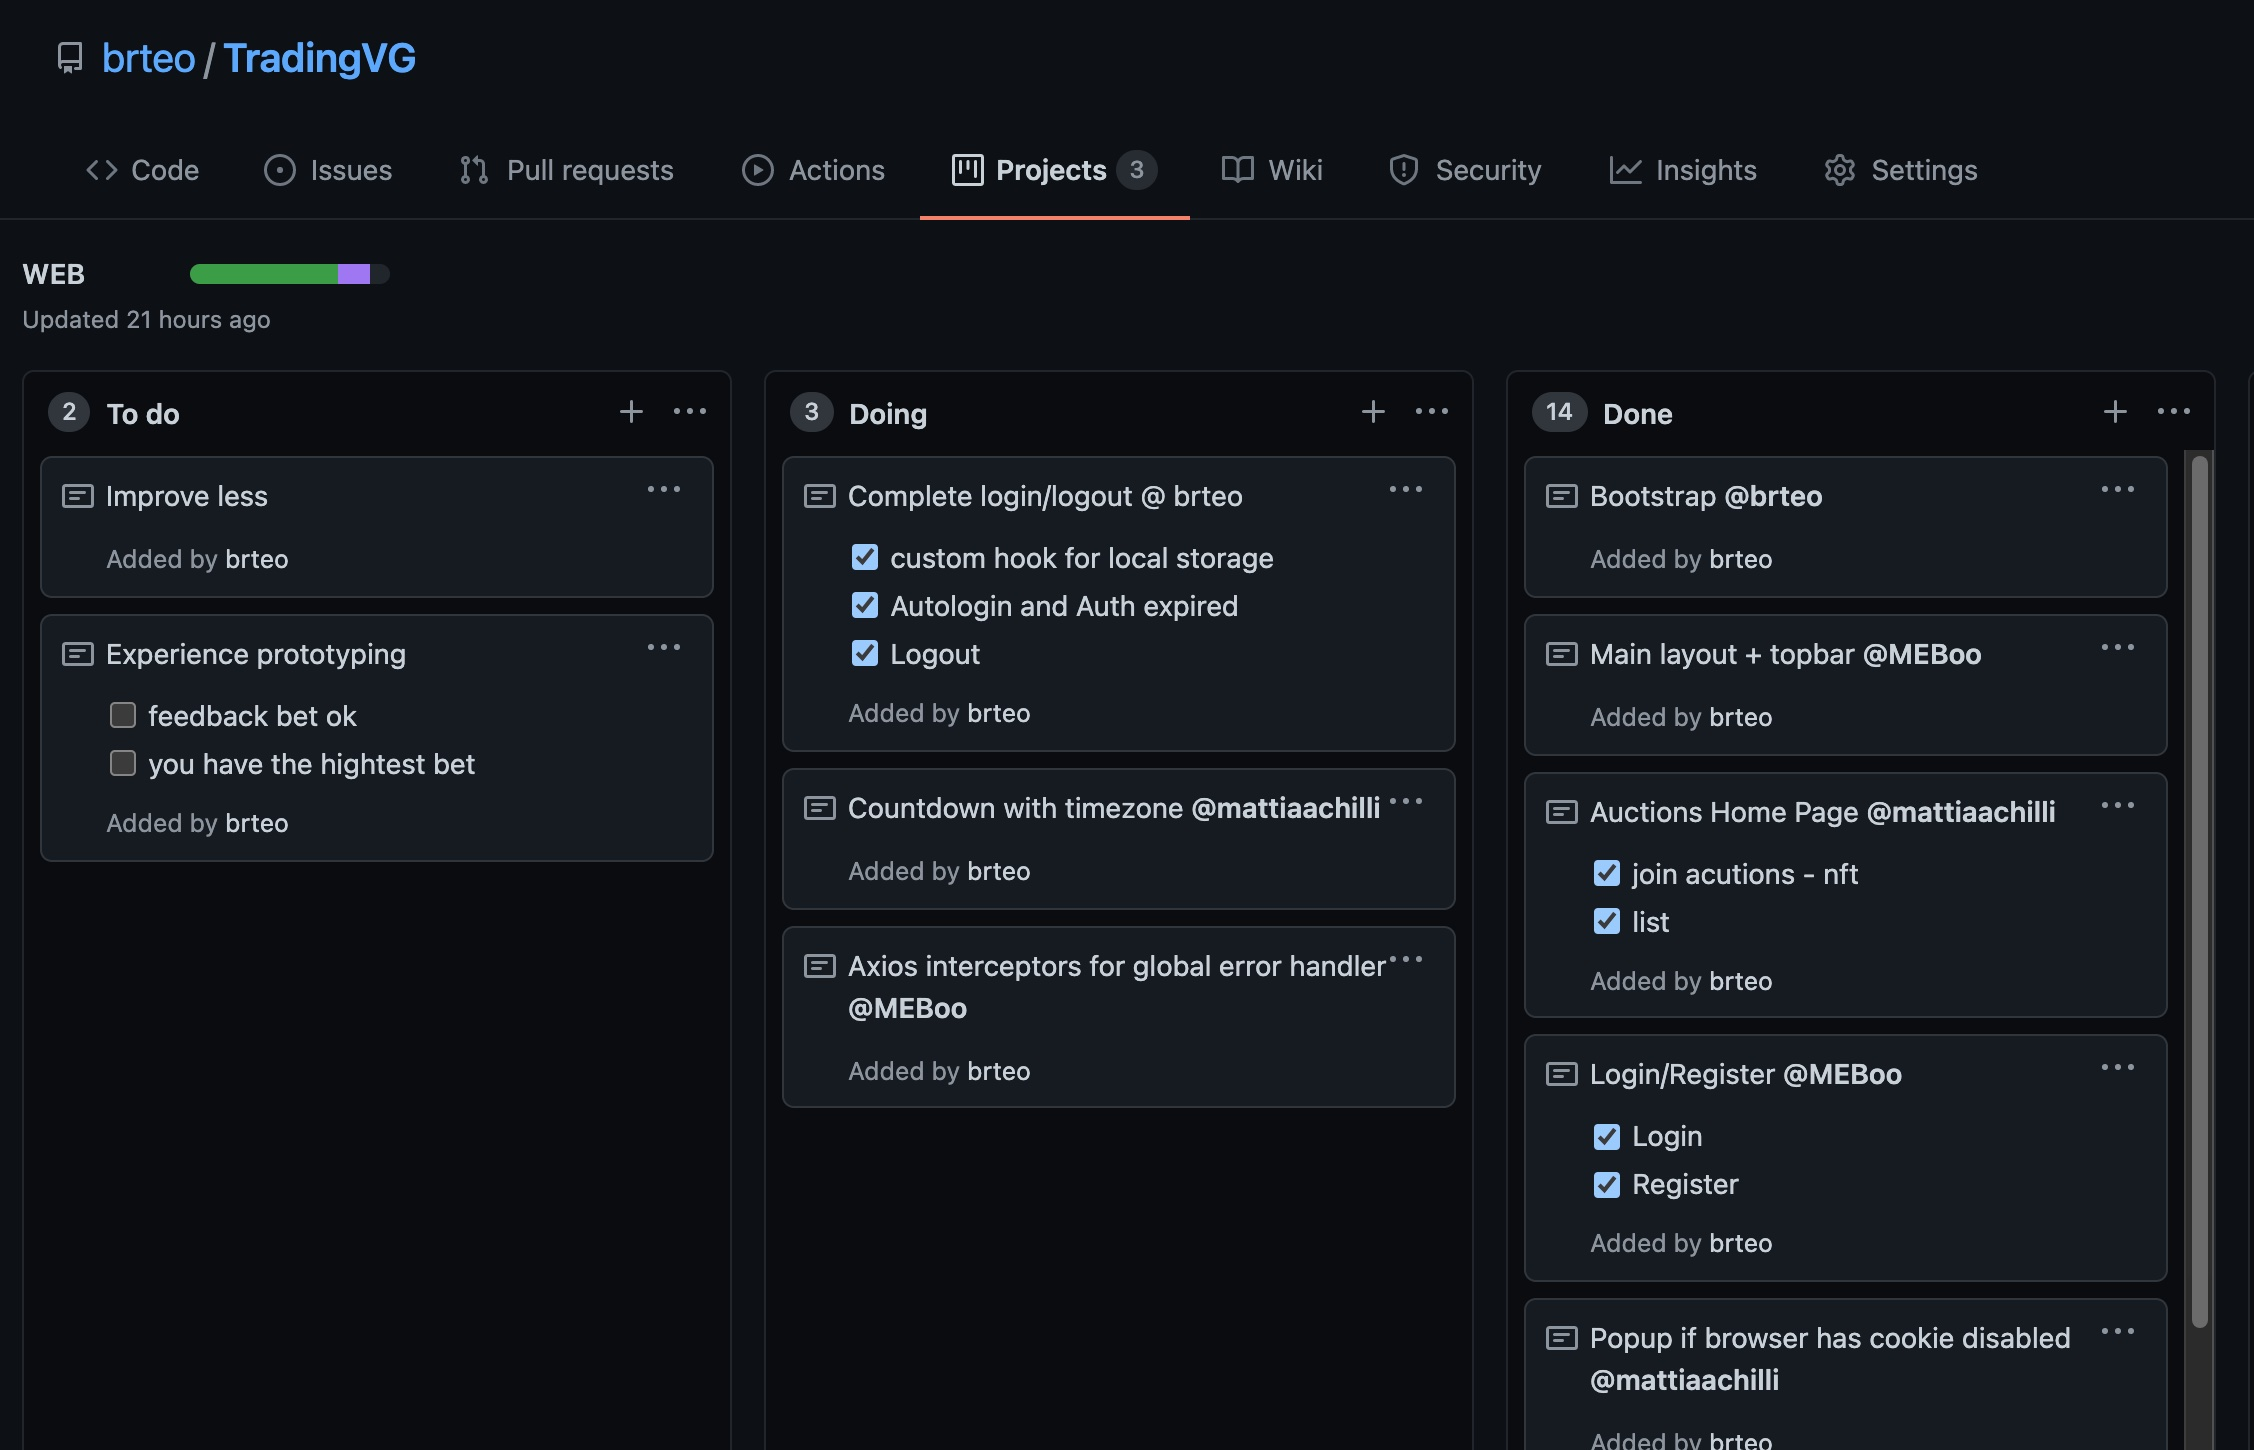
\includegraphics[width=\textwidth,keepaspectratio]{github-projects.jpg}
	\caption{GitHub Projects}
	\label{fig:github-projects}
\end{figure}

In questo modo siamo stati in grado di valutare progressivamente tutte le caratteristiche implementative ed accogliere i cambiamenti per tempo
dal momento che buona parte delle tecnologie si sono studiate durante la realizzazione del progetto.

Volendo utilizzare un approccio \textbf{User Centered Design}, durante l'intera fase di design e sviluppo,
ci si è focalizzati sui bisogni degli utenti al fine di creare un servizio che soddisfi gli utilizzatori.
In mancanza di utenti finali reali, durante le riunioni settimanali, 
il team valutava le funzionalità e l'interfaccia che stava prendendo forma immedesimandosi nelle \textbf{Personas} definite inizialmente [3.3.1].

Come strumento software a supporto si è deciso di utilizzare GitHub Projects all'interno del repository del progetto.

Infine abbiamo deciso fin dall'inizio di utilizzare il metodo \textbf{TDD} (Test Drive development) per quanto riguarda lo sviluppo della RestApi,
facendo in modo che tutti gli endpoint della RestApi siano oppurtunamente testati fin dall'inizio.

\clearpage

\subsection{Archittetura del sistema}
Dopo la definizione delle metodologie di sviluppo, ci siamo concentrati nella realizzazione dell'architettura del sistema.
Abbiamo immaginato che il portale web sia in futuro distribuito in moderne piattaforme cloud a microservizi.

\begin{figure}[H]
	\centering
	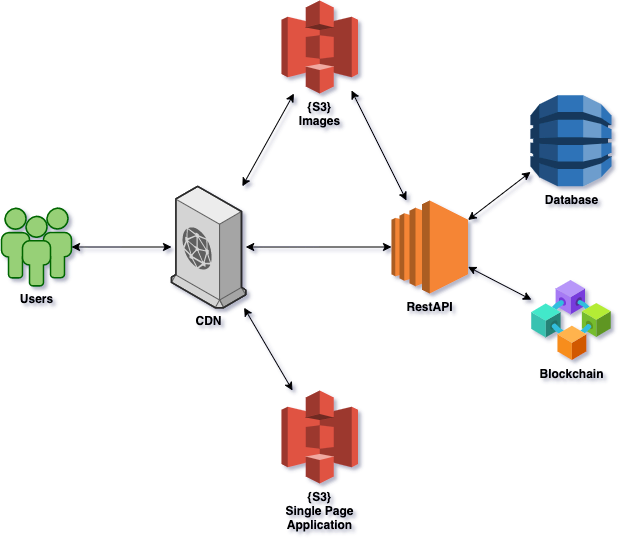
\includegraphics[width=0.75\textwidth,keepaspectratio]{architecture.png}
	\caption{Architettura del sistema}
	\label{fig:architecture}
\end{figure}

Gli utenti che navigheranno all'indirizzo web del portale accederanno alle risorse attraverso una \textbf{CDN} (Content Delivery Network),
una piattaforma di server altamente distribuita che aiuta a minimizzare il ritardo nel caricamento dei contenuti.

Il FrontEnd sarà una \textbf{SPA} (Single Page Application) ed in quanto tale potrà essere caricato su un Bucket \textbf{S3}. 
Le SPA sono applicazioni composte da una singola pagina non renderizzata lato server e
contenente tutto il codice necessario (HTML, JavaScript e CSS) recuperato in un singolo caricamento al prima accesso alla pagina.

Le altre risorse che compongono il portale saranno caricate dinamicamente secondo le esigenze attraverso chiamate al BackEnd dove sarà realizzata una RestApi 
che mette a disposizione attraverso i suoi EndPoint le azioni di tipo CRUD (Create, Read, Update, Delete) 
utili a reperire e manipolare le informazioni salvate su \textbf{Database}.

In questo progetto specifico si dovrà connetere la RestApi anche ad una \textbf{Blockchain} per la creazione e gestione degli NFT.
Le caratteristiche della Blockchain dovranno essere... quali Alan?

Infine le immagini saranno caricate su un'ulteriore Bucket \textbf{S3} per non appesantire la RestApi 
che deve restare sempre reattiva nello rispondere alle richieste degli utenti.

\clearpage

\subsection{Interfaccia utente}

\subsubsection{Target Users}
Chi sono e la loro storia

\subsubsection{Storyboard e Mockups}
Immagini e flussi principali

